%Folgende Zeile aktivieren und als SVN property "svn:keywords" auf "Id" setzen, um SVN Versionsinformationen im Dokument zu erhalten
%\svnInfo $Id: einleitung.tex 60 2012-01-26 15:56:06Z koppor $ 

\chapter{Beschreibung der zu untersuchenden Daten}
Die Ergebnisse der Messungen werden in zwei verschiedenen Formaten untersucht:

\begin{enumerate}
\item \textbf{3D-Voxeldaten} \\
In ihrer ursprünglichen Form liegen die Daten in Form von dreidimensionalen Rastergrafiken, zusammengesetzt aus volumetrischen Pixeln, vor. Diese Pixel werden üblicherweise als Voxel bezeichnet und sind Teil eines Voxelgitters. Jeder Voxel besitzt einen Wert, der seine Opazität wiedergibt. Der Wert dieser Opazität leitet sich direkt aus der beim CT gemessenen Reflektanzwert ab.

\begin{figure}[H]
  \begin{center}
    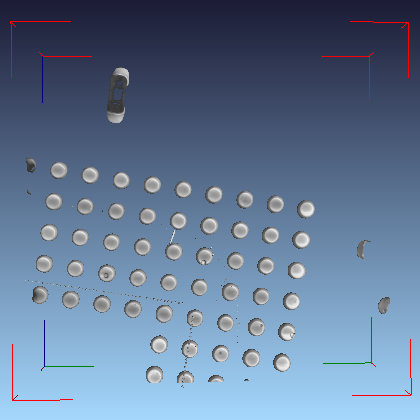
\includegraphics[width=0.5\textwidth]{3ddata.png}
    \caption{3D-Voxeldatensatz in myVGL}
    \label{fig:3ddata1}
  \end{center}
\end{figure}
\newpage
\item \textbf{2D-Slices} \\
Die zweidimensionalen Slices werden auf Basis der 3D-Voxeldaten berechnet. Dabei wird eine Schicht des Voxelgitters extrahiert und auf Basis der Opazitätswerte eine Rastergrafik erstellt, wobei jeder Pixel eindeutig einem Voxel zugeordnet werden kann. Durch diese Umformung können bei der Objekterkennung auch 2D-Verfahren genutzt werden.

\begin{figure}[H]
  \begin{center}
    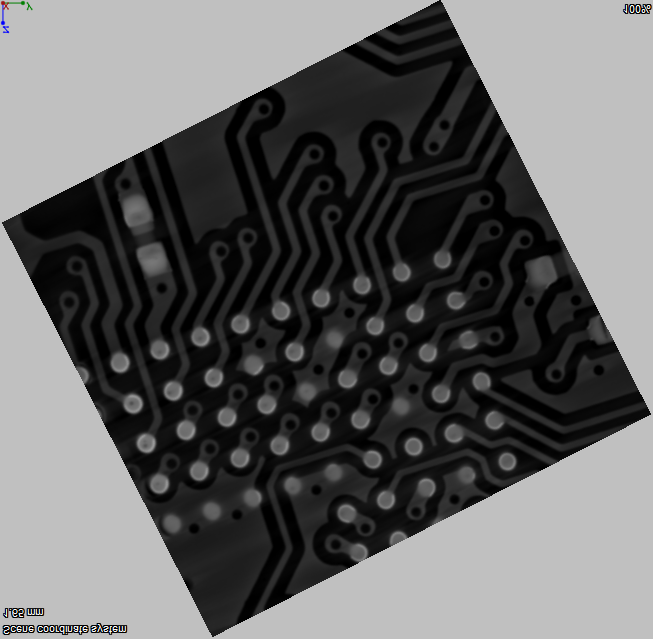
\includegraphics[width=0.5\textwidth]{2ddata.png}
    \caption{2D-Slice aus einem 3D-Voxeldatensatz}
    \label{fig:2ddata1}
  \end{center}
\end{figure}
\end{enumerate}

\begin{figure}[H]
  \begin{center}
    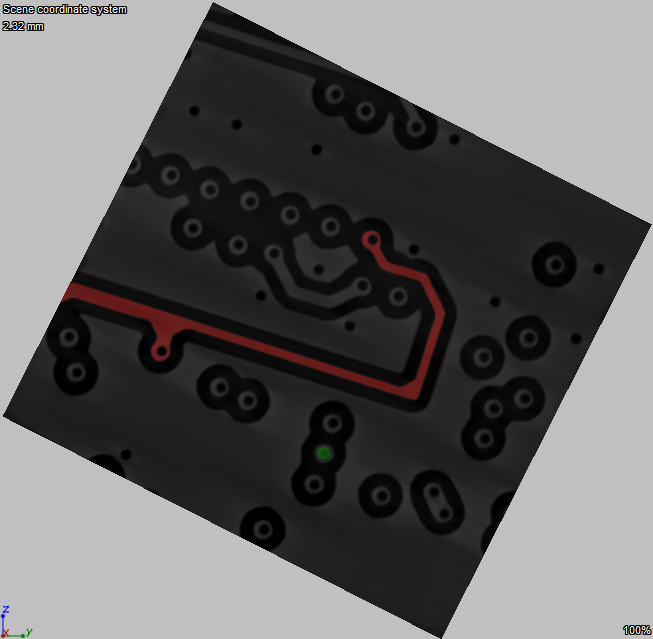
\includegraphics[width=0.5\textwidth]{zuerkennende.png}
    \caption{Typischer 2D-Slice mit Leiterbahnen (rot) und Bohrpunkten (grün)}
    \label{fig:zuerkennende1}
  \end{center}
\end{figure}

\section{Zu erkennende Objekte}

\subsection{Bohrpunkte}
Die Bohrpunkte sind die wohl am einfachsten zu erkennenden Objekte. Ihre Größe ist meistens durchweg identisch. Häufig münden Leiterbahnen in Bohrpunkten, manchmal befinden sie sich auch dazwischen, entlang des Körpers der Leiterbahn. Für dier Erkennung bietet es sich an auf den zweidimensionalen Slices zu arbeiten, weil die Bohrpunkte dort als schwarze, ausgefüllte Kreise leichter auszumachen sind.

\subsection{Leiterbahnen}
Die Leiterbahnen sind elektrisch leitende Verbindungen mit zweidimensionalem Verlauf. Aufgrund diesr Eigenschaft bietet es sich an wie bei den Bohrpunkten auf zweidimensionale Erkennungsverfahren zurückzugreifen. Da sie in den allermeisten Fällen an einem Bohrpunkt starten und auch wieder enden können diese gegebenenfalls auch als Ausgangspunkte für die Erkennung genutzt werden.

\begin{figure}[H]
  \begin{center}
    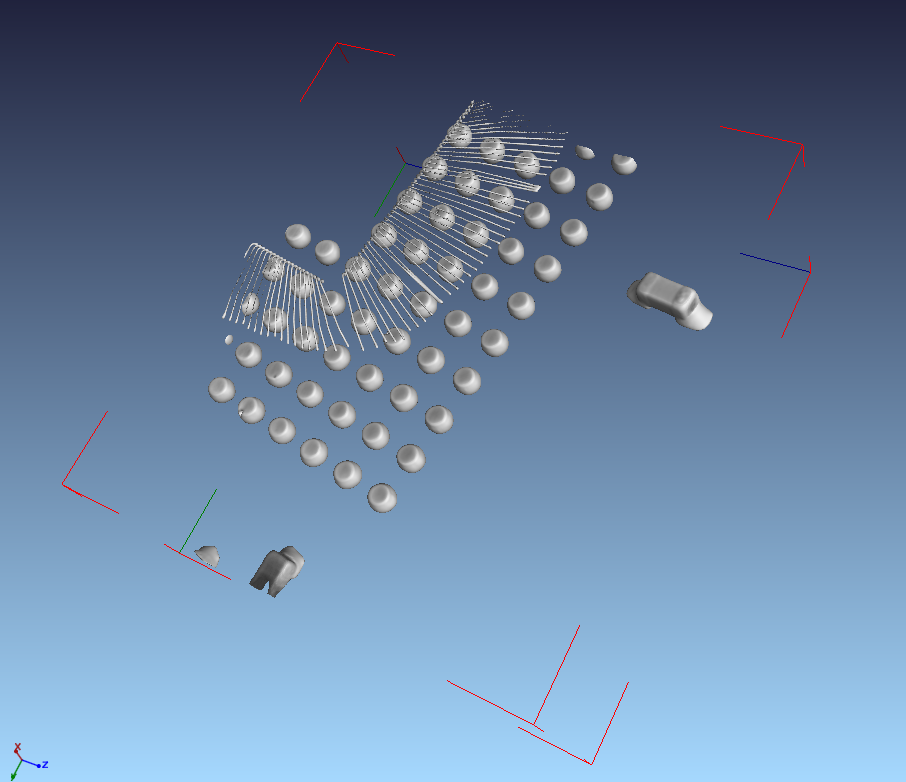
\includegraphics[width=0.9\textwidth]{BallsAndStuff.png}
    \caption{In der Mitte zu sehen: Bonddrähte und Lötkugeln}
    \label{fig:BallsAndBonds}
  \end{center}
\end{figure}

\subsection{Lötkugeln}
Die Lötkugeln sind die Objekte, die sich durch ihren Reflektanzwert am deutlichsten von anderen Objekten abheben. Deshalb können sie durch Filterung mit Threshholds sehr einfach vorisoliert werden. Die herausforderung besteht demnach darin die isolierten Voxel-Mengen auf Kugel-Eigenschaften zu untersuchen und gegebenenfalls als Lötkugel zu klassifizieren. Es sind allerdings auch Verfahren im zweidimensionalen denkbar, da die Kugelen auch auf den Slices sehr gut sichtbar sind. Dann wäre es allerdings nötig Schicht für Schicht, also Slice für Slice, vorzugehen und den Vorteil eines zusammenhängenden Objektes zu verwerfen.

\subsection{Bonddrähte}
Die Bonddrähte verbinden die Schichten der Platine, sie sind dünn und lang. Sie zeigen nicht unbedingt alle in die gleiche Richtung und weisen auch alle eine unterschiedliche Länge auf. Da sie im zweidimensionalen durch ihre geringe Größe und Erstreckung über mehrere Slices kaum erkennbar sind, müssen dreidimensinale Verfahren eingesetzt werden. Durch ihre undankbaren Eigenschaften sind sie die am schwersten zu erkennenden Objekte.